\documentclass[tikz,border=6pt]{standalone}
\usepackage{tikz}
\usepackage{amsmath,amssymb}
\usetikzlibrary{arrows.meta,positioning,shapes.geometric,fit,backgrounds,calc}

\definecolor{navy}{HTML}{1A365D}
\definecolor{darkblue}{HTML}{0F294A}
\definecolor{accentblue}{HTML}{2B6CB0}
\definecolor{softblue}{HTML}{EBF8FF}
\definecolor{darkred}{HTML}{C53030}
\definecolor{softred}{HTML}{FFF5F5}
\definecolor{darkgreen}{HTML}{22543D}
\definecolor{softgreen}{HTML}{F0FFF4}
\definecolor{darkgold}{HTML}{975A16}
\definecolor{softgold}{HTML}{FEFCBF}
\definecolor{darkgray}{HTML}{2D3748}

\begin{document}
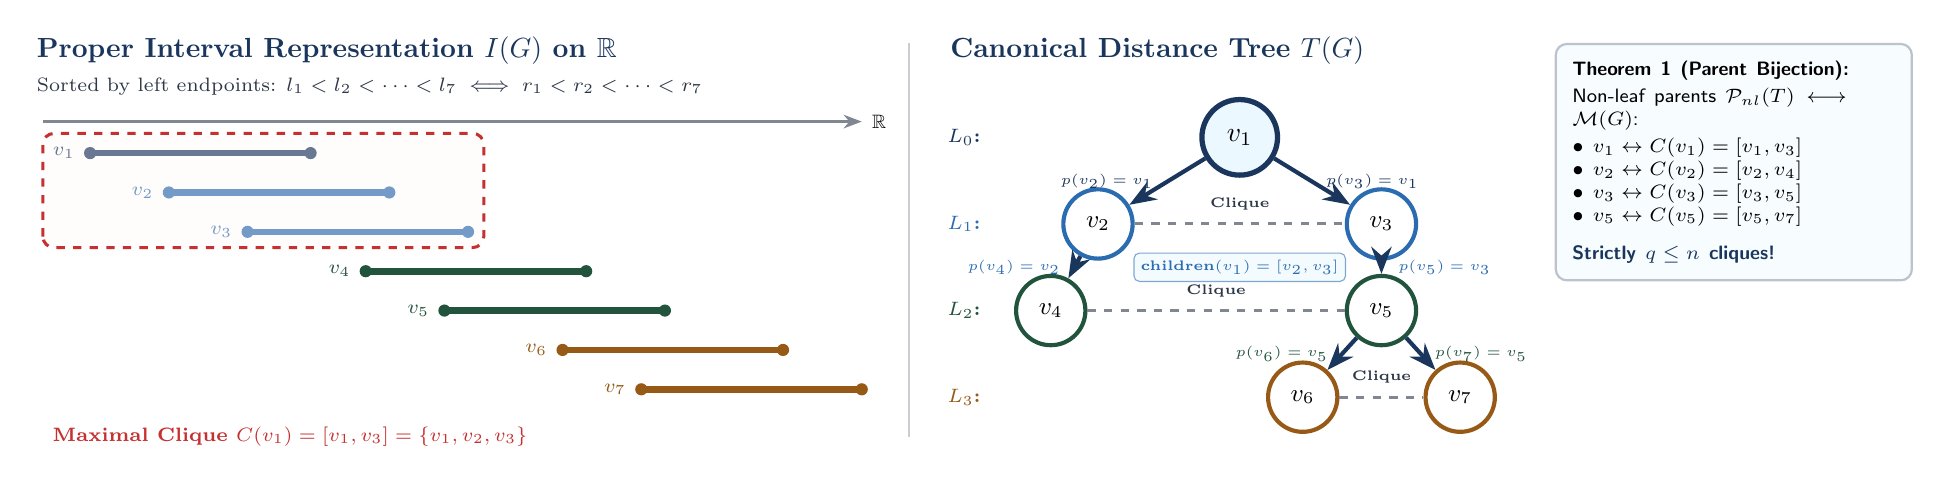
\begin{tikzpicture}[
    scale=1.0,
    >=Stealth,
    font=\sffamily,
    interval/.style={line width=2.4pt, line cap=round},
    treeNode/.style={circle, draw=navy, fill=white, line width=1.5pt, minimum size=0.88cm, inner sep=0pt, font=\bfseries\small},
    rootNode/.style={circle, draw=navy, fill=softblue, line width=1.9pt, minimum size=0.96cm, inner sep=0pt, font=\bfseries\normalsize},
    treeEdge/.style={->, line width=1.5pt, draw=navy},
    graphEdge/.style={-, dashed, line width=1.1pt, draw=darkgray!60}
]

    % ========================================================
    % LEFT PANEL: PROPER INTERVAL REPRESENTATION
    % ========================================================
    \node[anchor=west, font=\bfseries\normalsize, text=navy] at (0.0, 4.3) {\textbf{Proper Interval Representation $I(G)$ on $\mathbb{R}$}};
    \node[anchor=west, font=\scriptsize, text=darkgray] at (0.0, 3.85) {Sorted by left endpoints: $l_1 < l_2 < \dots < l_7 \iff r_1 < r_2 < \dots < r_7$};

    % Real Axis
    \draw[->, line width=0.8pt, draw=darkgray!60] (0.2, 3.4) -- (10.6, 3.4) node[right, font=\scriptsize\bfseries] {$\mathbb{R}$};

    % Intervals: clearly separated with distinct colours and labels
    \node[left=2pt, font=\scriptsize\bfseries, text=navy] at (0.8, 3.0) {$v_1$};
    \draw[interval, draw=navy] (0.8, 3.0) -- (3.6, 3.0);
    \fill[navy] (0.8, 3.0) circle (2.2pt); \fill[navy] (3.6, 3.0) circle (2.2pt);

    \node[left=2pt, font=\scriptsize\bfseries, text=accentblue] at (1.8, 2.5) {$v_2$};
    \draw[interval, draw=accentblue] (1.8, 2.5) -- (4.6, 2.5);
    \fill[accentblue] (1.8, 2.5) circle (2.2pt); \fill[accentblue] (4.6, 2.5) circle (2.2pt);

    \node[left=2pt, font=\scriptsize\bfseries, text=accentblue] at (2.8, 2.0) {$v_3$};
    \draw[interval, draw=accentblue] (2.8, 2.0) -- (5.6, 2.0);
    \fill[accentblue] (2.8, 2.0) circle (2.2pt); \fill[accentblue] (5.6, 2.0) circle (2.2pt);

    \node[left=2pt, font=\scriptsize\bfseries, text=darkgreen] at (4.3, 1.5) {$v_4$};
    \draw[interval, draw=darkgreen] (4.3, 1.5) -- (7.1, 1.5);
    \fill[darkgreen] (4.3, 1.5) circle (2.2pt); \fill[darkgreen] (7.1, 1.5) circle (2.2pt);

    \node[left=2pt, font=\scriptsize\bfseries, text=darkgreen] at (5.3, 1.0) {$v_5$};
    \draw[interval, draw=darkgreen] (5.3, 1.0) -- (8.1, 1.0);
    \fill[darkgreen] (5.3, 1.0) circle (2.2pt); \fill[darkgreen] (8.1, 1.0) circle (2.2pt);

    \node[left=2pt, font=\scriptsize\bfseries, text=darkgold] at (6.8, 0.5) {$v_6$};
    \draw[interval, draw=darkgold] (6.8, 0.5) -- (9.6, 0.5);
    \fill[darkgold] (6.8, 0.5) circle (2.2pt); \fill[darkgold] (9.6, 0.5) circle (2.2pt);

    \node[left=2pt, font=\scriptsize\bfseries, text=darkgold] at (7.8, 0.0) {$v_7$};
    \draw[interval, draw=darkgold] (7.8, 0.0) -- (10.6, 0.0);
    \fill[darkgold] (7.8, 0.0) circle (2.2pt); \fill[darkgold] (10.6, 0.0) circle (2.2pt);

    % Maximal Clique C(v1) = [v1, v3]
    \draw[draw=darkred, fill=softred, fill opacity=0.35, dashed, line width=1.1pt, rounded corners=4pt]
        (0.2, 1.8) rectangle (5.8, 3.25);
    \node[anchor=north west, text=darkred, font=\bfseries\scriptsize] at (0.2, -0.35) {Maximal Clique $C(v_1) = [v_1, v_3] = \{v_1, v_2, v_3\}$};

    % Panel Divider
    \draw[line width=0.8pt, draw=darkgray!25] (11.2, -0.6) -- (11.2, 4.4);

    % ========================================================
    % MIDDLE PANEL: CANONICAL DISTANCE TREE T(G)
    % ========================================================
    \node[anchor=west, font=\bfseries\normalsize, text=navy] at (11.6, 4.3) {\textbf{Canonical Distance Tree $T(G)$}};

    % Level indicators
    \node[font=\bfseries\scriptsize, text=navy] at (11.9, 3.2) {$L_0$:};
    \node[font=\bfseries\scriptsize, text=accentblue] at (11.9, 2.1) {$L_1$:};
    \node[font=\bfseries\scriptsize, text=darkgreen] at (11.9, 1.0) {$L_2$:};
    \node[font=\bfseries\scriptsize, text=darkgold] at (11.9, -0.1) {$L_3$:};

    % Tree Nodes
    \node[rootNode] (v1) at (15.4, 3.2) {$v_1$};

    \node[treeNode, draw=accentblue] (v2) at (13.6, 2.1) {$v_2$};
    \node[treeNode, draw=accentblue] (v3) at (17.2, 2.1) {$v_3$};

    \node[treeNode, draw=darkgreen] (v4) at (13.0, 1.0) {$v_4$};
    \node[treeNode, draw=darkgreen] (v5) at (17.2, 1.0) {$v_5$};

    \node[treeNode, draw=darkgold] (v6) at (16.2, -0.1) {$v_6$};
    \node[treeNode, draw=darkgold] (v7) at (18.2, -0.1) {$v_7$};

    % Clique edges (dashed)
    \draw[graphEdge] (v2) -- (v3) node[midway, above=1pt, font=\tiny\bfseries, text=darkgray] {Clique};
    \draw[graphEdge] (v4) -- (v5) node[midway, above=1pt, font=\tiny\bfseries, text=darkgray] {Clique};
    \draw[graphEdge] (v6) -- (v7) node[midway, above=1pt, font=\tiny\bfseries, text=darkgray] {Clique};

    % Tree Edges
    \draw[treeEdge] (v1) -- (v2) node[midway, left=1pt, font=\tiny\bfseries, text=navy] {$p(v_2)=v_1$};
    \draw[treeEdge] (v1) -- (v3) node[midway, right=1pt, font=\tiny\bfseries, text=navy] {$p(v_3)=v_1$};

    \draw[treeEdge] (v2) -- (v4) node[midway, left=1pt, font=\tiny\bfseries, text=accentblue] {$p(v_4)=v_2$};
    \draw[treeEdge] (v3) -- (v5) node[midway, right=2pt, font=\tiny\bfseries, text=accentblue] {$p(v_5)=v_3$};

    \draw[treeEdge] (v5) -- (v6) node[midway, left=1pt, font=\tiny\bfseries, text=darkgreen] {$p(v_6)=v_5$};
    \draw[treeEdge] (v5) -- (v7) node[midway, right=1pt, font=\tiny\bfseries, text=darkgreen] {$p(v_7)=v_5$};

    % Contiguous children indicator
    \node[draw=accentblue!60, fill=softblue!60, rounded corners=2pt, font=\tiny\bfseries, text=accentblue, inner sep=2.5pt] 
        at (15.4, 1.55) {$\text{children}(v_1)=[v_2, v_3]$};

    % ========================================================
    % RIGHT PANEL: PARENT BIJECTION SUMMARY CARD
    % ========================================================
    \node[draw=navy!30, fill=softblue!40, rounded corners=4pt, line width=0.8pt, anchor=north west, inner sep=6pt, text width=4.1cm] 
        at (19.4, 4.4) {
        \textbf{\scriptsize Theorem 1 (Parent Bijection):}\\
        \vspace{1.5pt}
        \fontsize{7.0}{8.3}\selectfont
        Non-leaf parents $\mathcal{P}_{nl}(T) \longleftrightarrow \mathcal{M}(G)$:\\
        \vspace{1.5pt}
        $\bullet$ $v_1 \leftrightarrow C(v_1) = [v_1, v_3]$\\
        $\bullet$ $v_2 \leftrightarrow C(v_2) = [v_2, v_4]$\\
        $\bullet$ $v_3 \leftrightarrow C(v_3) = [v_3, v_5]$\\
        $\bullet$ $v_5 \leftrightarrow C(v_5) = [v_5, v_7]$\\[2pt]
        \textbf{\color{navy}Strictly $q \le n$ cliques!}
    };

\end{tikzpicture}
\end{document}
